\subsection{Data Augmentation via Natural Weather Effects}
We augment our training data for an improved NN learning via natural-looking
weather effects alongside the usual data augmentation strategies.
\begin{itemize}
    \item \emph{light-rain:} A little blur to the image and random generated lines
    \item \emph{normal-rain:} Same as light-rain, but more lines
    \item \emph{snow:} Change the color of some part of picture to white to simulate snow.
    \item \emph{sun:} Increase brigthness for simulating a sunny day
\end{itemize}

We show these effects in action in Figure~\ref{fig:weather-effects}.

\begin{figure}
    \begin{subfigure}[b]{\textwidth}
        \centering
        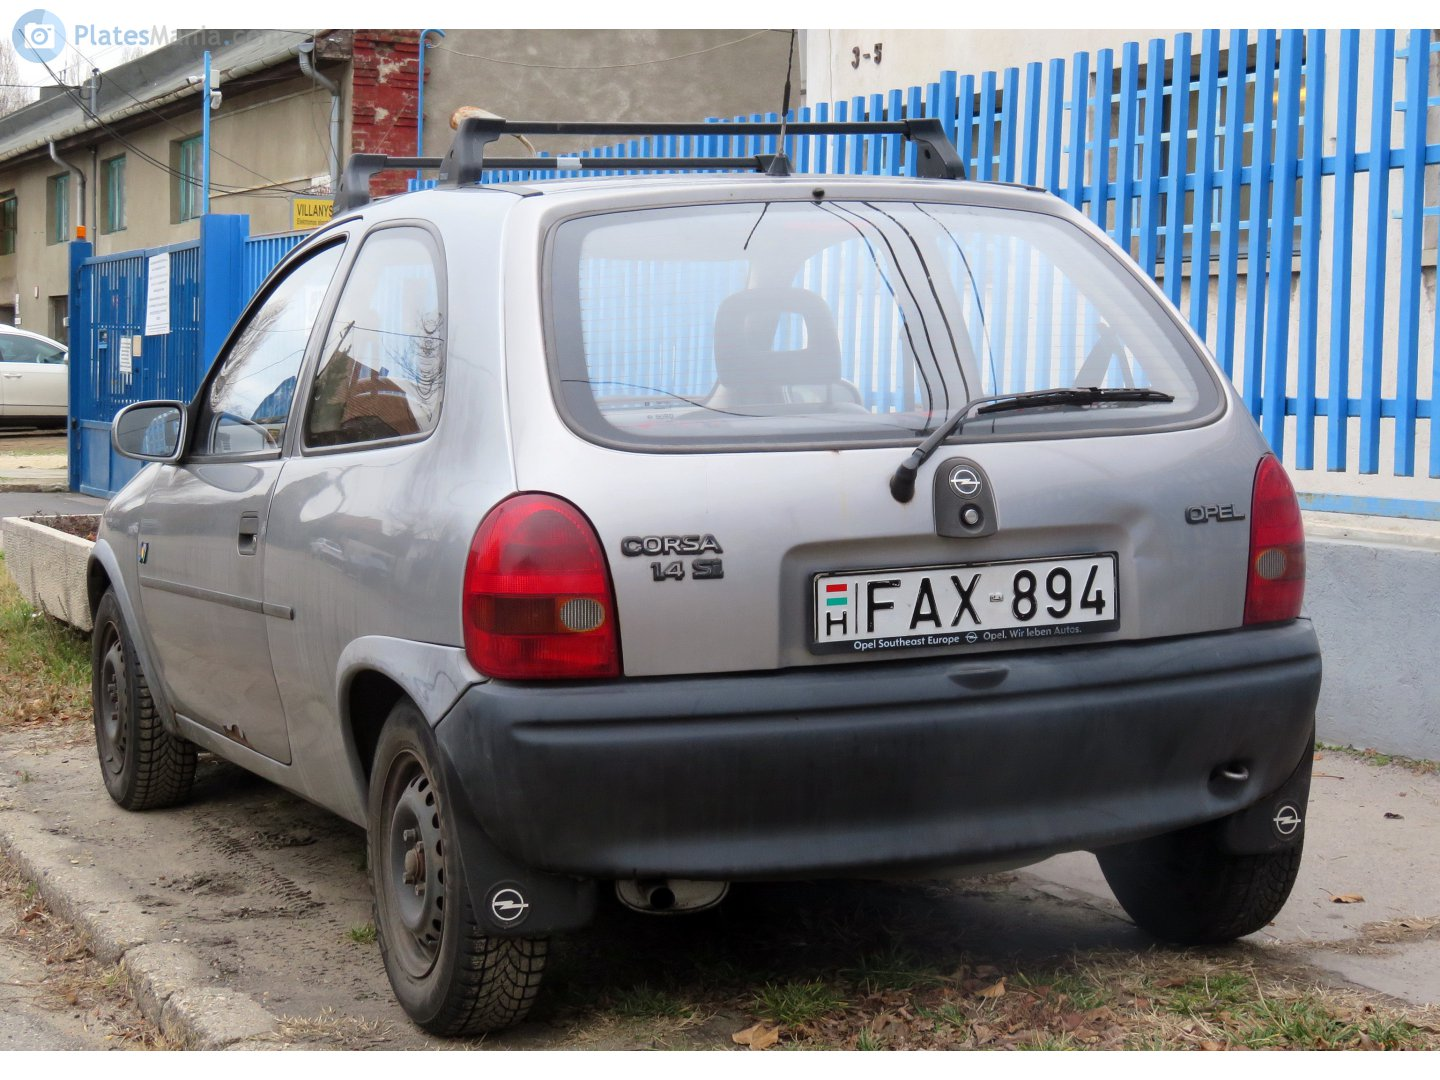
\includegraphics[width=0.45\textwidth]{figures/original.jpg}
        \caption{Original Image}
        \label{fig:weather-original}
    \end{subfigure}
    \begin{subfigure}[b]{\textwidth}
        \begin{subfigure}[b]{.45\textwidth}
            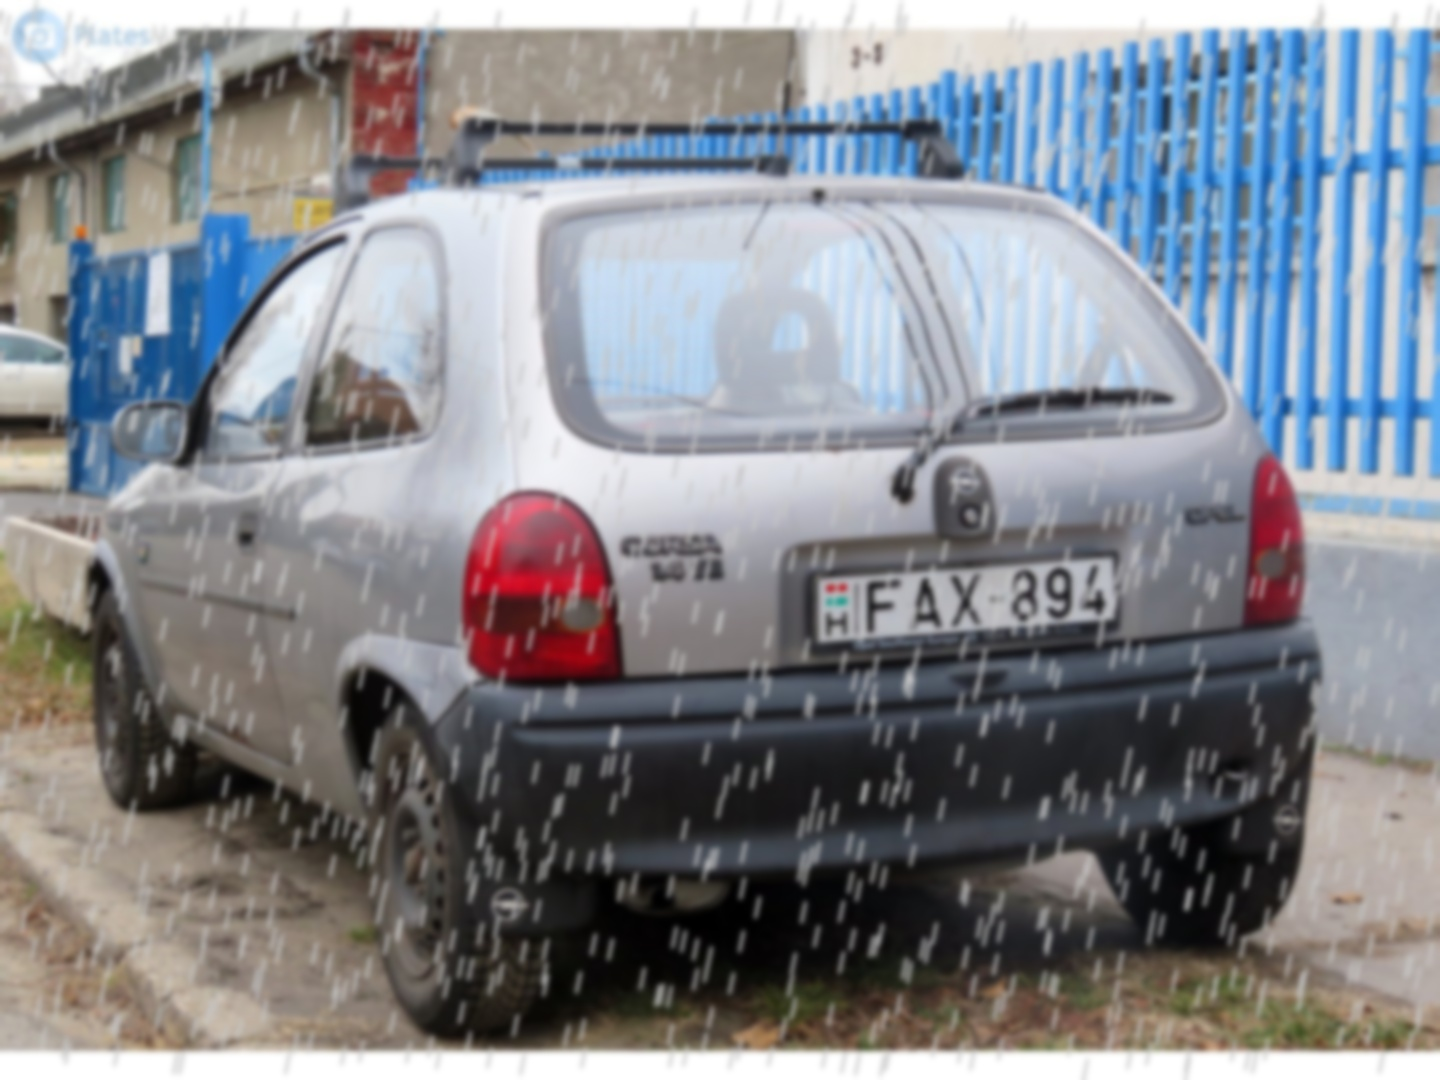
\includegraphics[width=\textwidth]{figures/lightrain.jpg}
        \end{subfigure}
        \hfill
        \begin{subfigure}[b]{.45\textwidth}
            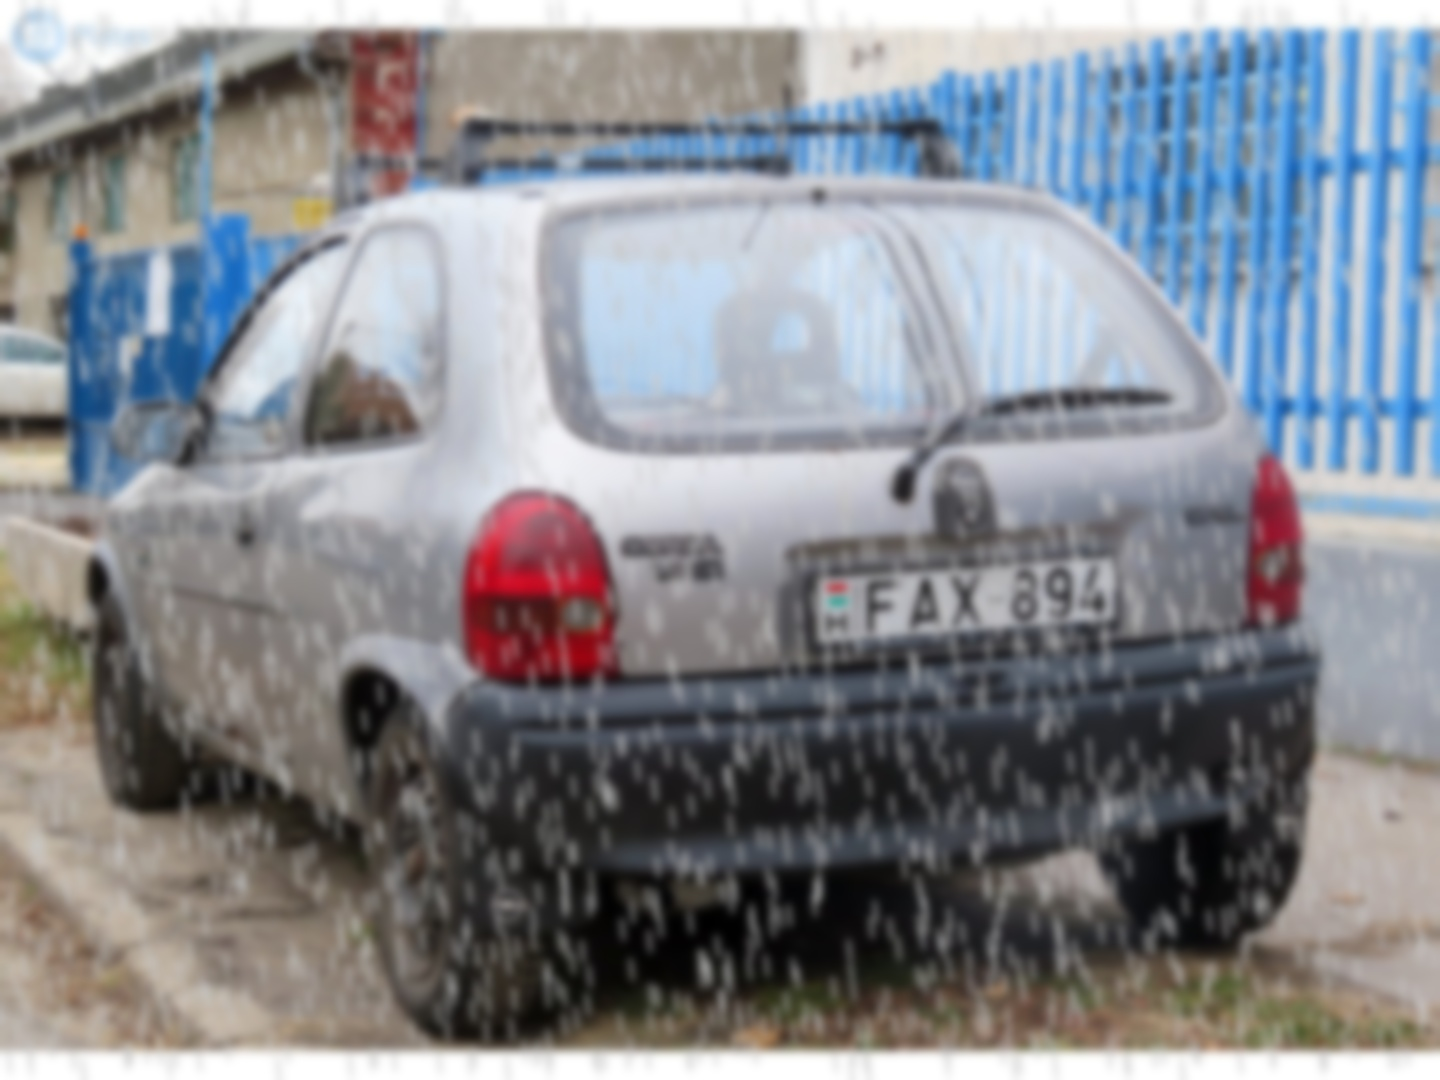
\includegraphics[width=\textwidth]{figures/rain.jpg}
        \end{subfigure}
        \hfill
        \caption{Two types of rain}
        \label{fig:weather-raines}
    \end{subfigure}
    \begin{subfigure}[b]{\textwidth}
        \begin{subfigure}[b]{.45\textwidth}
            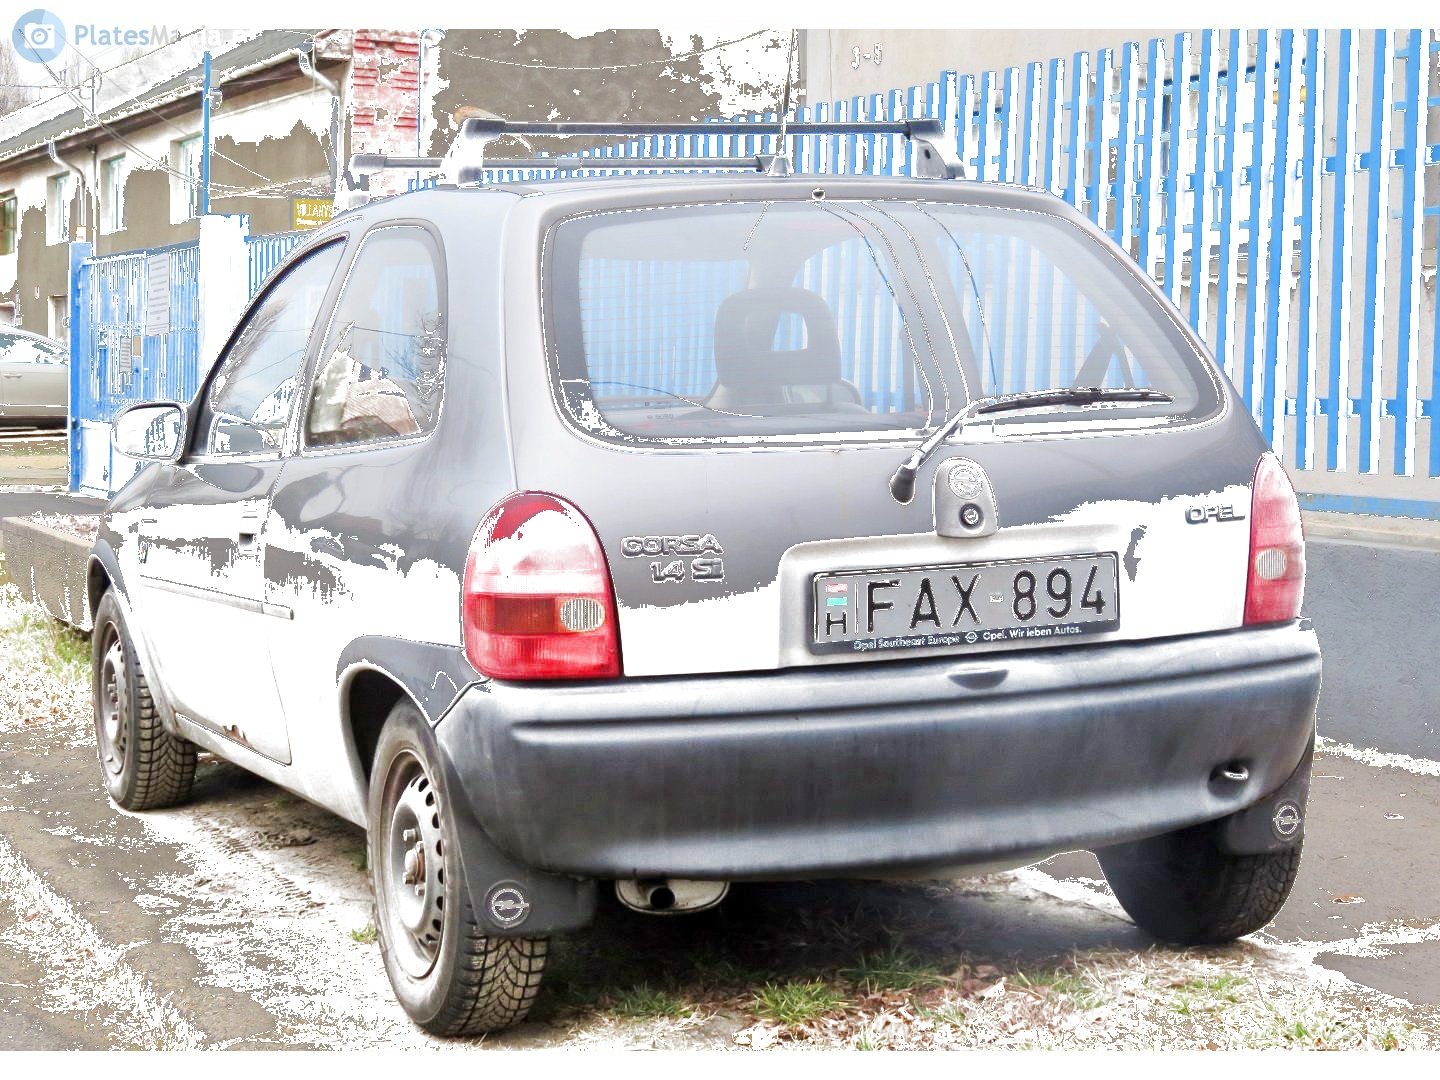
\includegraphics[width=\textwidth]{figures/snow.jpg}
        \end{subfigure}
        \hfill
        \begin{subfigure}[b]{.45\textwidth}
            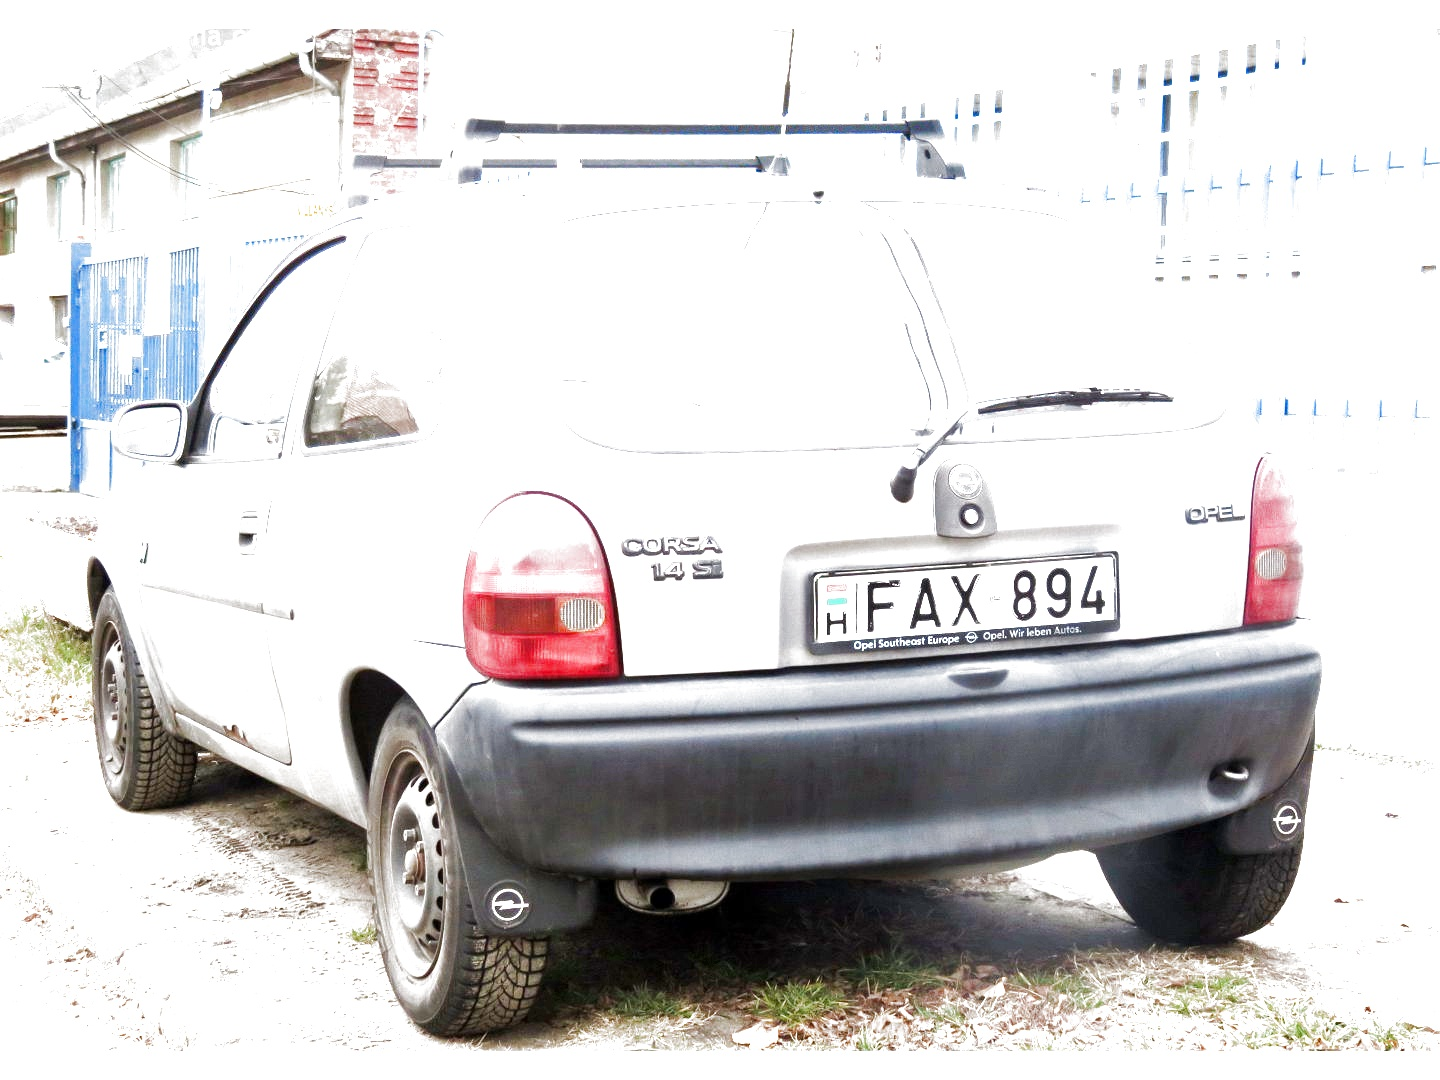
\includegraphics[width=\textwidth]{figures/sunny.jpg}
        \end{subfigure}
        \hfill
        \caption{Snow and Sun filter}
        \label{fig:weather-snow-sun}
    \end{subfigure}
    \caption{Different types of natural-looking weather effects.}
    \label{fig:weather-effects}
\end{figure}

Initially, we implemented these methods following this tutorial: 
\url{https://www.freecodecamp.org/news/image-augmentation-make-it-rain-make-it-snow-how-to-modify-a-photo-with-machine-learning-163c0cb3843f/}.

